% !TeX program = xelatex
% 学生：PDF1—6页；教师：PDF7—16页。A3横向，100%，双面短边翻转。
% 内容由同目录学生题目、知识清单、教师讲解三个文件输入，全部公式可编辑。
\documentclass[UTF8,fontset=windows,11pt,twocolumn]{ctexart}
\usepackage[paperwidth=420mm,paperheight=297mm,left=18mm,right=18mm,top=16mm,bottom=17mm,headheight=14pt]{geometry}
\setlength{\columnsep}{36mm}
\usepackage{amsmath,amssymb,array,booktabs,needspace,fancyhdr,tikz,eso-pic}
\usepackage[unicode,hidelinks]{hyperref}
\hypersetup{pdftitle={高一数学期中基础过关20题},pdfauthor={数学教学备课资料}}
\setlength{\parindent}{0pt}\setlength{\parskip}{3pt}
\linespread{1.1}\raggedbottom\setlength{\emergencystretch}{2em}
\pagestyle{fancy}\fancyhf{}\renewcommand{\headrulewidth}{0pt}
\newcommand{\Edition}{学生练习与知识清单}
\fancyfoot[C]{\small 期中基础过关20题\quad\Edition\quad 第\thepage 页}
\AddToShipoutPictureBG{\AtPageLowerLeft{\begin{tikzpicture}[remember picture,overlay]
\draw[black!25,dashed,line width=.25pt] (210mm,12mm)--(210mm,285mm);
\end{tikzpicture}}}
\newcommand{\subq}[2]{\par\Needspace{2\baselineskip}（#1）#2}
\newcommand{\score}[1]{（#1分）}
\newcommand{\field}[2]{\par\smallskip\textbf{#1：}#2\par}
\newcommand{\colhead}[2]{\noindent\begin{minipage}[t][20mm][t]{\linewidth}
\centering {\large\bfseries 高一数学期中基础过关20题}\par
{\small #1\quad #2}\par\end{minipage}\par}
\newsavebox{\statementbox}
\newcommand{\exercise}[2]{\sbox{\statementbox}{\begin{minipage}{\linewidth}
\textbf{#1.（10分）}#2\end{minipage}}%
\typeout{QUESTIONHEIGHT #1=\the\dimexpr\ht\statementbox+\dp\statementbox\relax}%
\noindent\begin{minipage}[t][12cm][t]{\linewidth}\usebox{\statementbox}\par\vfill\end{minipage}\par}
\newcommand{\readinggraph}{\begin{center}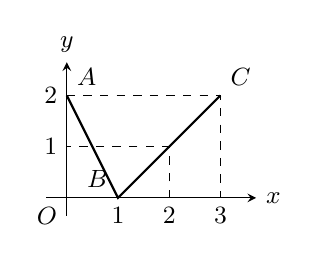
\begin{tikzpicture}[x=.65cm,y=.65cm,>=stealth,font=\small]
\draw[->](-.4,0)--(3.7,0)node[right]{$x$};\draw[->](0,-.35)--(0,2.65)node[above]{$y$};
\draw[thick](0,2)node[above right]{$A$}--(1,0)node[above left]{$B$}--(3,2)node[above right]{$C$};
\draw[dashed](0,2)--(3,2)--(3,0);\draw[dashed](2,0)--(2,1)--(0,1);
\node[below left]at(0,0){$O$};\foreach \x in {1,2,3}\node[below]at(\x,0){$\x$};
\foreach \y in {1,2}\node[left]at(0,\y){$\y$};\end{tikzpicture}\end{center}}

\begin{document}
\pdfbookmark[0]{学生练习20题}{student}
\colhead{学生练习}{第1—2题\quad 每题10分}
\exercise{1}{设全集 $U=\{-2,-1,0,1,2,3,4\}$，集合 $A=\{x\in\mathbb Z\mid-1\le x\le2\}$，$B=\{0,2,4\}$。\subq{1}{用列举法表示 $A$；}\subq{2}{求 $A\cap B$ 和 $A\cup B$；}\subq{3}{求 $\complement_U B$，并分别判断 $0\in A$、$\{0,2\}\subseteq A$ 是否成立。}}
\exercise{2}{设 $U=\mathbb R$，$A=\{x\mid x\le1\}$，$B=\{x\mid t<x<4\}$，其中 $t<4$。\subq{1}{当 $t=-2$ 时，求 $A\cap B$、$A\cup B$ 和 $\complement_U A$；}\subq{2}{若 $A\cup B=(-\infty,4)$，求 $t$ 的取值范围。}}
\newpage
\colhead{学生练习}{第3—4题\quad 每题10分}
\exercise{3}{设 $x\in\mathbb R$，分别判断下列两个条件之间的充分、必要关系，并说明理由。\subq{1}{$p$：$x=1$；$q$：$x^2=1$。判断 $p$ 是 $q$ 的什么条件；}\subq{2}{$r$：$x^2\le4$；$s$：$|x|\le2$。判断 $r$ 是 $s$ 的什么条件。}}
\exercise{4}{已知命题 $p$：$\forall x\in[0,+\infty)$，$x^2+1>0$；命题 $q$：$\exists x\in\mathbb R$，$x^2+1<0$。\subq{1}{写出命题p的否定；}\subq{2}{写出命题q的否定；}\subq{3}{判断p、q的真假，并说明理由。}}
\newpage
\colhead{学生练习}{第5—6题\quad 每题10分}
\exercise{5}{已知 $a>b>0$，$c<0$。\subq{1}{比较 $ac$ 与 $bc$、$\dfrac1a$ 与 $\dfrac1b$ 的大小；}\subq{2}{比较 $a^2c$ 与 $b^2c$ 的大小；}\subq{3}{“对任意 $d\in\mathbb R$，均有 $ad^2>bd^2$”是否正确？若不正确，给出反例，并写出对所有实数d都成立的大小关系及等号成立的条件。}}
\exercise{6}{解下列关于x的不等式，第（3）问中 $m\in\mathbb R$。\subq{1}{$-x^2+3x+4>0$；}\subq{2}{$(2x-1)^2\le9$；}\subq{3}{$(x-m)(x-1)\le0$。}}
\newpage
\colhead{学生练习}{第7—8题\quad 每题10分}
\exercise{7}{求下列最值，并写出取到最值时自变量的值。\subq{1}{当 $x>1$ 时，求 $x+\dfrac9{x-1}$ 的最小值；}\subq{2}{当 $0<x<8$ 时，求 $\sqrt{x(8-x)}$ 的最大值。}}
\exercise{8}{已知 $m\in\mathbb R$。\subq{1}{若对任意 $x\in\mathbb R$，都有 $x^2-4x+m\ge0$，求m的取值范围；}\subq{2}{若将第（1）问中的“$\ge0$”改为“$>0$”，求m的取值范围。}}
\newpage
\colhead{学生练习}{第9—10题\quad 每题10分}
\exercise{9}{回答下列问题，每问都说明理由。\subq{1}{$y=\sqrt{x^2}$ 与 $y=|x|$ 是否表示同一个函数？}\subq{2}{$y=x$ 与 $y=\dfrac{x^2}{x}$ 是否表示同一个函数？}\subq{3}{设 $A=\{-1,0,1\}$，$B=\{0,1,2\}$。对应 $x\mapsto x^2$ 能否构成从A到B的函数？它的值域是否等于B？}}
\exercise{10}{求下列函数的定义域。\subq{1}{$f(x)=\dfrac{\sqrt{3-x}}{x-1}$；}\subq{2}{$g(x)=\sqrt{x-1}+\dfrac1{x-3}$。}}
\newpage
\colhead{学生练习}{第11—12题\quad 每题10分}
\exercise{11}{已知 $f(x)=\begin{cases}x+2,&x\le0,\\x^2,&x>0.\end{cases}$\subq{1}{求 $f(0)$、$f(-1)$ 和 $f(f(-1))$；}\subq{2}{函数g的对应关系如下表，求 $g(g(2))$。\par\smallskip\begin{tabular}{c|ccc}$x$&1&2&3\\\hline$g(x)$&3&1&2\end{tabular}}\subq{3}{若对任意 $x\in\mathbb R$ 都有 $h(x+2)=2x-1$，求 $h(3)$，并求 $h(x)$ 的解析式。}}
\exercise{12}{函数 $y=f(x)$ 的图象为折线ABC，$A(0,2)$、$B(1,0)$、$C(3,2)$。\readinggraph\subq{1}{写出f的定义域和值域；}\subq{2}{求 $f(0)$ 和 $f(f(0))$；}\subq{3}{求不等式 $f(x)\le1$ 的解集。}}
\newpage
\colhead{学生练习}{第13—14题\quad 每题10分}
\exercise{13}{已知函数 $f(x)=x^2-2x$，$x\in[-1,3]$。\subq{1}{写出f的单调递减区间和单调递增区间；}\subq{2}{求f的最大值、最小值，并写出取得各最值时x的所有取值；}\subq{3}{写出f的值域。}}
\exercise{14}{完成下列问题。\subq{1}{用定义证明函数 $f(x)=x^2$ 在 $[0,+\infty)$ 上单调递增；}\subq{2}{若函数 $h(x)=x^2-2ax$ 在 $(-\infty,3]$ 上单调递减，求实数a的取值范围。}}
\newpage
\colhead{学生练习}{第15—16题\quad 每题10分}
\exercise{15}{已知f是定义在 $\mathbb R$ 上的奇函数，当 $x\ge0$ 时，$f(x)=x^2+2x$。\subq{1}{求 $f(0)$ 和 $f(-2)$；}\subq{2}{求f在 $(-\infty,0)$ 上的解析式；}\subq{3}{将 $f(-3)$、$f(-1)$、$f(2)$ 按从小到大排列。}}
\exercise{16}{已知g的定义域为 $[-2,2]$，设 $f(x)=g(x)+g(-x)$。当 $x\in[0,2]$ 时，$f(x)=2x-x^2$。\subq{1}{判断f的奇偶性，并证明；}\subq{2}{求f在 $[-2,0)$ 上的解析式；}\subq{3}{求f在 $[-2,2]$ 上的最大值、最小值，并写出所有最值点的横坐标。}}
\newpage
\colhead{学生练习}{第17—18题\quad 每题10分}
\exercise{17}{计算下列各式，写出必要步骤。\subq{1}{$32^{\frac25}+27^{-\frac23}$；}\subq{2}{$16^{\frac34}+8^{-\frac23}$；}\subq{3}{$\sqrt{(-3)^2}+\sqrt[3]{-8}$。}}
\exercise{18}{已知幂函数 $f(x)=x^\alpha$ 的图象经过点 $\left(4,\dfrac1{16}\right)$。\subq{1}{求f的解析式及定义域；}\subq{2}{判断f的奇偶性，并写出它的单调区间及增减性；}\subq{3}{用定义证明f在 $(0,+\infty)$ 上单调递减；}\subq{4}{分别写出函数 $h(x)=x^{3/2}$、$k(x)=x^{-1/2}$ 的实数定义域。}}
\newpage
\colhead{学生练习}{第19—20题\quad 每题10分}
\exercise{19}{已知指数函数 $f(x)=a^x$ 的图象经过点 $(2,4)$，其中 $a>0$ 且 $a\ne1$，设 $g(x)=a^{|x-1|}$。\subq{1}{求a的值；}\subq{2}{写出g的单调区间及相应的增减性，并求g的值域；}\subq{3}{解不等式 $g(x)\le8$。}}
\exercise{20}{某种物质的剩余量 $M(t)$（g）满足 $M(t)=100a^t$，其中t为经过的时间（年），$t\ge0$，$a>0$ 且 $a\ne1$。已知两年后剩余25 g。\subq{1}{求a和 $M(t)$ 的解析式；}\subq{2}{判断 $M(t)$ 的单调性，写出值域，并说明剩余量能否等于0；}\subq{3}{当剩余量不少于12.5 g时，求t的取值范围。}}
\newpage

\pdfbookmark[0]{20题对应知识清单}{knowledge}
\colhead{对应知识清单}{第1—10题}
\field{第1题}{元素与集合用 $\in$；集合与集合用 $\subseteq$。交集取公共元素，并集取所有元素，补集必须相对于全集。}
\field{第2题}{区间的开闭端点表示能否取到。并集恰好等于给定区间，要同时做到无遗漏、无超出；连接点只需由一个集合覆盖。}
\field{第3题}{$p\Rightarrow q$ 时p是q的充分条件，q是p的必要条件；两方向均能推出才是充要。否定某个推出关系，只需一个反例。}
\field{第4题}{全称命题的否定改用存在量词，存在命题的否定改用全称量词；量词范围保持不变。$>$ 的否定是 $\le$，$<$ 的否定是 $\ge$。}
\field{第5题}{同加减保序；乘除正数保序，乘除负数反向。非负不等于正，$d^2$ 在 $d=0$ 时为0。}
\field{第6题}{先统一为正的二次项系数，再找根、画数轴、判端点。含参根须比较顺序；重根时回到原不等式判断。}
\field{第7题}{对非负数u、v，有 $u+v\ge2\sqrt{uv}$，等号当且仅当 $u=v$。求最值必须检查正负条件、定值结构和等号可取性。}
\field{第8题}{对所有x都非负，等价于可取得的最小值非负；对所有x都为正，须结合最小值是否取得判断。二次式配方后可直接找最值。}
\field{第9题}{函数要求定义域中每个数都有唯一像；允许多个自变量有相同函数值。相同函数须定义域、对应关系都相同，值域是实际取到的像的集合。}
\field{第10题}{偶次根式的被开方数须非负，分母须非零；多个限制同时满足，取交集。根号内等于0时，还要检查分母。}
\newpage
\colhead{对应知识清单}{第11—20题}
\field{第11题}{求 $f(f(a))$ 先求内层，再把结果作为新输入；分段函数每次都要重新选段。已知 $h(x+c)$ 时，先看括号内整体。}
\field{第12题}{定义域看图象覆盖的横坐标，值域看纵坐标；读函数值先找横坐标。图象解不等式时，要保留水平线交点并结合原定义域。}
\field{第13题}{二次函数先配方找对称轴，再与定义域比较。闭区间最值须检查顶点是否在内以及两端点；求出所有取等位置，值域写成集合。}
\field{第14题}{定义证明须任取区间内两个有大小顺序的数，作差、变形、定号并下结论。二次函数区间单调问题取决于对称轴的位置。}
\field{第15题}{奇函数定义域关于原点对称，满足 $f(-x)=-f(x)$；若0在定义域中，则 $f(0)=0$。已知半轴解析式时先把输入变到已知半轴。}
\field{第16题}{$g(x)+g(-x)$ 的定义域需使两个输入均合法；在对称域内它是偶函数。利用轴对称补出另一半图象及全部最值点。}
\field{第17题}{正底数有 $a^{m/n}=(\sqrt[n]a)^m$，$a^{-r}=1/a^r$。$\sqrt{u^2}=|u|$；奇次实根保留被开方数的符号。}
\field{第18题}{幂函数由给定点确定指数，再按原式求定义域。奇偶性先查对称域；单调区间不能跨越无定义点。负分数指数还须排除根式为0。}
\field{第19题}{指数函数底数须大于0且不为1；底数大于1时保序，介于0与1时反序。带绝对值的指数先找分界点，再看内外两层的增减。}
\field{第20题}{指数模型必须保留实际定义域。衰减模型底数介于0与1之间；同底指数比较反向；趋近0与实际等于0不同。}

\clearpage
\renewcommand{\Edition}{教师讲解、评分与教材出处}
\pdfbookmark[0]{教师讲解与教材出处}{teacher}
\colhead{教师讲解与评分}{第1题\quad 10分}
\textbf{题目}\quad 设全集 $U=\{-2,-1,0,1,2,3,4\}$，集合 $A=\{x\in\mathbb Z\mid-1\le x\le2\}$，$B=\{0,2,4\}$。\subq{1}{用列举法表示 $A$；}\subq{2}{求 $A\cap B$ 和 $A\cup B$；}\subq{3}{求 $\complement_U B$，并分别判断 $0\in A$、$\{0,2\}\subseteq A$ 是否成立。}
\field{知识点}{元素与集合用 $\in$；集合与集合用 $\subseteq$。交集取公共元素，并集取所有元素，补集必须相对于全集。}
\field{分步解答}{\subq{1}{$A=\{-1,0,1,2\}$。\score{2}}\subq{2}{同时在两集合中的元素是0、2，故 $A\cap B=\{0,2\}$（2分）；合并所有元素并去重，$A\cup B=\{-1,0,1,2,4\}$（2分）。}\subq{3}{在 $U$ 中删去0、2、4，得 $\complement_U B=\{-2,-1,1,3\}$（2分）。$0\in A$ 成立（1分）；0、2均在A中，故 $\{0,2\}\subseteq A$ 成立（1分）。}}
\field{书写顺序}{先列举，再逐元素检查，最后核对全集。}
\field{易错提醒}{把0遗漏；把属于与包含混写；在全集外取补。}
\field{独立达标}{四个集合结果正确，能解释两种关系符号的对象。}
{\footnotesize\field{教材母题}{p.13，习题1.1第8题（教材PDF第20页）\par{\ttfamily\detokenize{XJ-B1-C01-HW-P013-Y0307}}\par p.13，习题1.1第9题（教材PDF第20页）\par{\ttfamily\detokenize{XJ-B1-C01-HW-P013-Y0433}}}\field{改编说明}{将教材有限集合运算改为整数描述集，合并元素与子集判断。}\field{教材帮对应知识}{S01：书内p.1、2（PDF10、11页）；S02：书内p.2、3、4（PDF11、12、13页）；S03：书内p.11、12、13（PDF20、21、22页）；S04：书内p.19、20（PDF28、29页）；S05：书内p.21（PDF30页）}}
\newpage
\colhead{教师讲解与评分}{第2题\quad 10分}
\textbf{题目}\quad 设 $U=\mathbb R$，$A=\{x\mid x\le1\}$，$B=\{x\mid t<x<4\}$，其中 $t<4$。\subq{1}{当 $t=-2$ 时，求 $A\cap B$、$A\cup B$ 和 $\complement_U A$；}\subq{2}{若 $A\cup B=(-\infty,4)$，求 $t$ 的取值范围。}
\field{知识点}{区间的开闭端点表示能否取到。并集恰好等于给定区间，要同时做到无遗漏、无超出；连接点只需由一个集合覆盖。}
\field{分步解答}{\subq{1}{$A\cap B=(-2,1]$（2分），$A\cup B=(-\infty,4)$（2分），$\complement_U A=(1,+\infty)$（2分）。}\subq{2}{当 $t\le1$ 时，1由A覆盖，两集合连接且覆盖所有小于4的数（2分）；当 $t>1$ 时，$(1,t]$ 未被覆盖，故不满足。所求 $t\le1$，即 $(-\infty,1]$（2分）。}}
\field{书写顺序}{在同一数轴上标出两集合，先检查连接点，再反查参数边界。}
\field{易错提醒}{看到B左端开就删除参数等号；漏掉补集端点。}
\field{独立达标}{独立写出t=1为何仍成立，并说明t>1漏掉哪里。}
{\footnotesize\field{教材母题}{p.13，习题1.1第9题（教材PDF第20页）\par{\ttfamily\detokenize{XJ-B1-C01-HW-P013-Y0433}}\par p.13，习题1.1第16题（教材PDF第20页）\par{\ttfamily\detokenize{XJ-B1-C01-HW-P013-Y1442}}}\field{改编说明}{将教材集合运算与参数关系题改为数轴上的区间连接。}\field{教材帮对应知识}{S02：书内p.2、3、4（PDF11、12、13页）；S03：书内p.11、12、13（PDF20、21、22页）；S04：书内p.19、20（PDF28、29页）；S05：书内p.21（PDF30页）}}
\newpage
\colhead{教师讲解与评分}{第3题\quad 10分}
\textbf{题目}\quad 设 $x\in\mathbb R$，分别判断下列两个条件之间的充分、必要关系，并说明理由。\subq{1}{$p$：$x=1$；$q$：$x^2=1$。判断 $p$ 是 $q$ 的什么条件；}\subq{2}{$r$：$x^2\le4$；$s$：$|x|\le2$。判断 $r$ 是 $s$ 的什么条件。}
\field{知识点}{$p\Rightarrow q$ 时p是q的充分条件，q是p的必要条件；两方向均能推出才是充要。否定某个推出关系，只需一个反例。}
\field{分步解答}{\subq{1}{$x=1\Rightarrow x^2=1$（2分），但 $x=-1$ 满足q而不满足p（2分），故p是q的充分而不必要条件（1分）。}\subq{2}{$x^2\le4\Leftrightarrow-2\le x\le2$（2分）；$|x|\le2$ 也等价于 $-2\le x\le2$（2分）。两者能互相推出，r是s的充要条件（1分）。}}
\field{书写顺序}{每次都检查正向和反向，不能凭语感给名称。}
\field{易错提醒}{把必要与充分的方向写反；只检查一个方向。}
\field{独立达标}{能画两方向箭头，并为不成立的方向给出反例。}
{\footnotesize\field{教材母题}{p.18，例5（教材PDF第25页）\par{\ttfamily\detokenize{XJ-B1-C01-EX-P018-Y0491}}}\field{改编说明}{将教材充分必要关系判断改为两组最简单的实数条件。}\field{教材帮对应知识}{L02：书内p.30、31（PDF39、40页）}}
\newpage
\colhead{教师讲解与评分}{第4题\quad 10分}
\textbf{题目}\quad 已知命题 $p$：$\forall x\in[0,+\infty)$，$x^2+1>0$；命题 $q$：$\exists x\in\mathbb R$，$x^2+1<0$。\subq{1}{写出命题p的否定；}\subq{2}{写出命题q的否定；}\subq{3}{判断p、q的真假，并说明理由。}
\field{知识点}{全称命题的否定改用存在量词，存在命题的否定改用全称量词；量词范围保持不变。$>$ 的否定是 $\le$，$<$ 的否定是 $\ge$。}
\field{分步解答}{\subq{1}{$\exists x\in[0,+\infty)$，$x^2+1\le0$。量词改为存在，范围不变，不等号同时否定。\score{3}}\subq{2}{$\forall x\in\mathbb R$，$x^2+1\ge0$。\score{3}}\subq{3}{任意实数x都有 $x^2\ge0$，所以 $x^2+1\ge1>0$。p为真命题（2分）；不存在实数使 $x^2+1<0$，q为假命题（2分）。}}
\field{书写顺序}{依次改量词、保范围、否定结论，再独立判断原命题真假。}
\field{易错提醒}{把否定写成反命题；把>的否定写成<；扩大变量范围。}
\field{独立达标}{两条否定中量词、范围、不等号三处均正确。}
{\footnotesize\field{教材母题}{p.23，页首练习（教材PDF第30页）\par{\ttfamily\detokenize{XJ-B1-C01-PR-P023-Y0176}}}\field{改编说明}{保留教材量词否定结构，补充真假判断以检查概念理解。}\field{教材帮对应知识}{L03：书内p.38、39（PDF47、48页）；L04：书内p.39、40（PDF48、49页）}}
\newpage
\colhead{教师讲解与评分}{第5题\quad 10分}
\textbf{题目}\quad 已知 $a>b>0$，$c<0$。\subq{1}{比较 $ac$ 与 $bc$、$\dfrac1a$ 与 $\dfrac1b$ 的大小；}\subq{2}{比较 $a^2c$ 与 $b^2c$ 的大小；}\subq{3}{“对任意 $d\in\mathbb R$，均有 $ad^2>bd^2$”是否正确？若不正确，给出反例，并写出对所有实数d都成立的大小关系及等号成立的条件。}
\field{知识点}{同加减保序；乘除正数保序，乘除负数反向。非负不等于正，$d^2$ 在 $d=0$ 时为0。}
\field{分步解答}{\subq{1}{乘以负数要反向，$ac<bc$（2分）。$\frac1a-\frac1b=\frac{b-a}{ab}<0$，故 $\frac1a<\frac1b$（2分）。}\subq{2}{由 $a>b>0$ 得 $a^2>b^2$，再乘负数c，得 $a^2c<b^2c$。\score{3}}\subq{3}{不正确，取 $d=0$，两边都为0（1分）。由 $(a-b)d^2\ge0$ 得 $ad^2\ge bd^2$（1分），且等号当且仅当 $d=0$ 时成立（1分）。}}
\field{书写顺序}{先看乘除量的符号；不能由大小关系直接对任意实数平方。}
\field{易错提醒}{乘负数不反向；以为任意实数的平方都大于0。}
\field{独立达标}{每次比较都指出符号依据，并写出d=0这个反例。}
{\footnotesize\field{教材母题}{p.37，练习第1题（教材PDF第44页）\par{\ttfamily\detokenize{XJ-B1-C02-PR-P037-Y0875}}\par p.43，习题2.1第3题（教材PDF第50页）\par{\ttfamily\detokenize{XJ-B1-C02-HW-P043-Y0634}}}\field{改编说明}{将教材不等式性质判断改为直接写关系与反例。}\field{教材帮对应知识}{I01：书内p.44（PDF53页）；I02：书内p.45、46（PDF54、55页）}}
\newpage
\colhead{教师讲解与评分}{第6题\quad 10分}
\textbf{题目}\quad 解下列关于x的不等式，第（3）问中 $m\in\mathbb R$。\subq{1}{$-x^2+3x+4>0$；}\subq{2}{$(2x-1)^2\le9$；}\subq{3}{$(x-m)(x-1)\le0$。}
\field{知识点}{先统一为正的二次项系数，再找根、画数轴、判端点。含参根须比较顺序；重根时回到原不等式判断。}
\field{分步解答}{\subq{1}{原式等价于 $(x+1)(x-4)<0$（1分），两根之间取负，故解集为 $(-1,4)$（2分）。}\subq{2}{$-3\le2x-1\le3$（1分），所以 $-1\le x\le2$，解集为 $[-1,2]$（2分）。}\subq{3}{乘积非正取两根之间并包含两根（1分）。$m<1$ 时解集为 $[m,1]$（1分）；$m=1$ 时为 $\{1\}$（1分）；$m>1$ 时为 $[1,m]$（1分）。}}
\field{书写顺序}{因式分解或转为双边不等式；第3问按m与1的大小分三类。}
\field{易错提醒}{乘-1漏反向；把$\le$写成开区间；重根时误答空集或全R。}
\field{独立达标}{三问都以解集收尾，且能直接代入检验重根分支。}
{\footnotesize\field{教材母题}{p.59，习题2.3第4题（教材PDF第66页）\par{\ttfamily\detokenize{XJ-B1-C02-HW-P059-Y0221}}\par p.59，习题2.3第8题（教材PDF第66页）\par{\ttfamily\detokenize{XJ-B1-C02-HW-P059-Y0874}}}\field{改编说明}{合并教材二次不等式基础解法与单参数根序分类，先给出因式。}\field{教材帮对应知识}{I02：书内p.45、46（PDF54、55页）；I04：书内p.64、65、66（PDF73、74、75页）}}
\newpage
\colhead{教师讲解与评分}{第7题\quad 10分}
\textbf{题目}\quad 求下列最值，并写出取到最值时自变量的值。\subq{1}{当 $x>1$ 时，求 $x+\dfrac9{x-1}$ 的最小值；}\subq{2}{当 $0<x<8$ 时，求 $\sqrt{x(8-x)}$ 的最大值。}
\field{知识点}{对非负数u、v，有 $u+v\ge2\sqrt{uv}$，等号当且仅当 $u=v$。求最值必须检查正负条件、定值结构和等号可取性。}
\field{分步解答}{\subq{1}{令 $t=x-1>0$，原式为 $1+t+9/t$（1分）。由基本不等式 $t+9/t\ge2\sqrt9=6$（2分），原式最小值为7（1分），等号在 $t=3$，即 $x=4$ 时取得（1分）。}\subq{2}{两数x与 $8-x$ 为正，且和为8（1分），故 $x(8-x)\le((x+8-x)/2)^2=16$（2分）。根式最大值为4（1分），等号在 $x=8-x$，即 $x=4$ 时取得，且满足原范围（1分）。}}
\field{书写顺序}{第1问把x改写为(x-1)+1，第2问识别定和。}
\field{易错提醒}{只写一个界不写取等点；把x与x-1误当相同量。}
\field{独立达标}{两问都写清比较量、最值和可行取等点。}
{\footnotesize\field{教材母题}{p.43，习题2.1第7题（教材PDF第50页）\par{\ttfamily\detokenize{XJ-B1-C02-HW-P043-Y1506}}}\field{改编说明}{将教材基本不等式最值题分为定积求和、定和求积两种短问。}\field{教材帮对应知识}{I03：书内p.52、53、54（PDF61、62、63页）}}
\newpage
\colhead{教师讲解与评分}{第8题\quad 10分}
\textbf{题目}\quad 已知 $m\in\mathbb R$。\subq{1}{若对任意 $x\in\mathbb R$，都有 $x^2-4x+m\ge0$，求m的取值范围；}\subq{2}{若将第（1）问中的“$\ge0$”改为“$>0$”，求m的取值范围。}
\field{知识点}{对所有x都非负，等价于可取得的最小值非负；对所有x都为正，须结合最小值是否取得判断。二次式配方后可直接找最值。}
\field{分步解答}{\subq{1}{$x^2-4x+m=(x-2)^2+m-4$（2分）。最小值在 $x=2$ 时为 $m-4$（1分）。恒非负等价于 $m-4\ge0$，故 $m\in[4,+\infty)$（2分）。}\subq{2}{最小值 $m-4$ 必须严格为正（2分），故 $m>4$，即 $(4,+\infty)$（2分）。当 $m=4,x=2$ 时原式等于0，不能取端点4（1分）。}}
\field{书写顺序}{把全称量词转为最小值条件，再用端点代入检验。}
\field{易错提醒}{把恒成立当成有解；忽略严格与非严格的不等号差别。}
\field{独立达标}{说明为何取x=2即可检查必要性，并解释m=4的差异。}
{\footnotesize\field{教材母题}{p.55，例5（教材PDF第62页）\par{\ttfamily\detokenize{XJ-B1-C02-EX-P055-Y0177}}}\field{改编说明}{在教材恒成立母题中更换数据，对比严格与非严格条件。}\field{教材帮对应知识}{I06：书内p.71、72、73（PDF80、81、82页）；F06：书内p.99、83、84（PDF108、92、93页）}}
\newpage
\colhead{教师讲解与评分}{第9题\quad 10分}
\textbf{题目}\quad 回答下列问题，每问都说明理由。\subq{1}{$y=\sqrt{x^2}$ 与 $y=|x|$ 是否表示同一个函数？}\subq{2}{$y=x$ 与 $y=\dfrac{x^2}{x}$ 是否表示同一个函数？}\subq{3}{设 $A=\{-1,0,1\}$，$B=\{0,1,2\}$。对应 $x\mapsto x^2$ 能否构成从A到B的函数？它的值域是否等于B？}
\field{知识点}{函数要求定义域中每个数都有唯一像；允许多个自变量有相同函数值。相同函数须定义域、对应关系都相同，值域是实际取到的像的集合。}
\field{分步解答}{\subq{1}{是。两者定义域都为 $\mathbb R$（1分），且对任意实数x，$\sqrt{x^2}=|x|$，对应关系相同（2分）。}\subq{2}{不是。前者定义域为 $\mathbb R$（1分），后者为 $\mathbb R\setminus\{0\}$，定义域不同，约分不能补回0（2分）。}\subq{3}{能。A中每个元素都有唯一平方，且像均在B中（2分）。实际值域为 $\{0,1\}$（1分），不是B；函数不要求取遍B的每个元素（1分）。}}
\field{书写顺序}{先查定义域，再查每个输入的对应值，不只看式子能否化简。}
\field{易错提醒}{约分后补回0；误以为像集必须取遍给定集合B。}
\field{独立达标}{能分别用定义域和对应关系作判断，并区分B与值域。}
{\footnotesize\field{教材母题}{p.77，习题3.1第5题（教材PDF第84页）\par{\ttfamily\detokenize{XJ-B1-C03-HW-P077-Y0403}}\par p.67，练习第1题（教材PDF第74页）\par{\ttfamily\detokenize{XJ-B1-C03-PR-P067-Y0874}}}\field{改编说明}{把教材函数本质及相同函数选择判断改为写理由的主观题。}\field{教材帮对应知识}{F01：书内p.77、78（PDF86、87页）；F02：书内p.79、80、81（PDF88、89、90页）}}
\newpage
\colhead{教师讲解与评分}{第10题\quad 10分}
\textbf{题目}\quad 求下列函数的定义域。\subq{1}{$f(x)=\dfrac{\sqrt{3-x}}{x-1}$；}\subq{2}{$g(x)=\sqrt{x-1}+\dfrac1{x-3}$。}
\field{知识点}{偶次根式的被开方数须非负，分母须非零；多个限制同时满足，取交集。根号内等于0时，还要检查分母。}
\field{分步解答}{\subq{1}{须同时满足 $3-x\ge0$、$x-1\ne0$（2分），即 $x\le3$ 且 $x\ne1$（1分）。定义域为 $(-\infty,1)\cup(1,3]$（2分）。}\subq{2}{须 $x-1\ge0$ 且 $x-3\ne0$（2分），即 $x\ge1$、$x\ne3$（1分）。定义域为 $[1,3)\cup(3,+\infty)$（2分）。}}
\field{书写顺序}{先逐项列限制，再联立，最后用区间表示。}
\field{易错提醒}{把根式条件写成严格>0；遗漏分母非零；把交集写成并集。}
\field{独立达标}{两问都保留可取的根式端点并排除分母零点。}
{\footnotesize\field{教材母题}{p.77，习题3.1第4题（教材PDF第84页）\par{\ttfamily\detokenize{XJ-B1-C03-HW-P077-Y0286}}}\field{改编说明}{更换教材定义域母题中的根式与分母数据，形成两种方向。}\field{教材帮对应知识}{F02：书内p.79、80、81（PDF88、89、90页）}}
\newpage
\colhead{教师讲解与评分}{第11题\quad 10分}
\textbf{题目}\quad 已知 $f(x)=\begin{cases}x+2,&x\le0,\\x^2,&x>0.\end{cases}$\subq{1}{求 $f(0)$、$f(-1)$ 和 $f(f(-1))$；}\subq{2}{函数g的对应关系如下表，求 $g(g(2))$。\par\smallskip\begin{tabular}{c|ccc}$x$&1&2&3\\\hline$g(x)$&3&1&2\end{tabular}}\subq{3}{若对任意 $x\in\mathbb R$ 都有 $h(x+2)=2x-1$，求 $h(3)$，并求 $h(x)$ 的解析式。}
\field{知识点}{求 $f(f(a))$ 先求内层，再把结果作为新输入；分段函数每次都要重新选段。已知 $h(x+c)$ 时，先看括号内整体。}
\field{分步解答}{\subq{1}{0归第一段，$f(0)=2$（1分）；$f(-1)=1$（1分）；外层输入变为正数1，应用第二段，$f(f(-1))=f(1)=1$（2分）。}\subq{2}{先查得 $g(2)=1$（1分），再查得 $g(1)=3$，故 $g(g(2))=3$（2分）。}\subq{3}{令 $x=1$ 得 $h(3)=1$（1分）。令 $u=x+2$，则 $x=u-2$，所以 $h(u)=2(u-2)-1=2u-5$（1分），即 $h(x)=2x-5\ (x\in\mathbb R)$（1分）。}}
\field{书写顺序}{由内向外逐层代入；表格逐次查找；解析式可换元。}
\field{易错提醒}{外层沿用内层所用分段；把h(3)误算成2×3-1。}
\field{独立达标}{能写出外层为什么换段，并准确完成换元。}
{\footnotesize\field{教材母题}{p.76，练习第2题（教材PDF第83页）\par{\ttfamily\detokenize{XJ-B1-C03-PR-P076-Y0364}}\par p.78，习题3.1第11题（教材PDF第85页）\par{\ttfamily\detokenize{XJ-B1-C03-HW-P078-Y0473}}\par p.90，复习题第3题（教材PDF第97页）\par{\ttfamily\detokenize{XJ-B1-C03-RV-P090-Y0678}}}\field{改编说明}{合并教材分段求值、查表复合求值和换元求解析式三类短问。}\field{教材帮对应知识}{F03：书内p.80、87、88、89、90、131（PDF89、96、97、98、99、140页）；F04：书内p.85、86、93、94（PDF94、95、102、103页）；F07：书内p.86、91、92、93（PDF95、100、101、102页）}}
\newpage
\colhead{教师讲解与评分}{第12题\quad 10分}
\textbf{题目}\quad 函数 $y=f(x)$ 的图象为折线ABC，$A(0,2)$、$B(1,0)$、$C(3,2)$。\readinggraph\subq{1}{写出f的定义域和值域；}\subq{2}{求 $f(0)$ 和 $f(f(0))$；}\subq{3}{求不等式 $f(x)\le1$ 的解集。}
\field{知识点}{定义域看图象覆盖的横坐标，值域看纵坐标；读函数值先找横坐标。图象解不等式时，要保留水平线交点并结合原定义域。}
\field{分步解答}{\subq{1}{图象横坐标取遍 $[0,3]$，故定义域为 $[0,3]$（1分）；纵坐标取遍 $[0,2]$，故值域为 $[0,2]$（2分）。}\subq{2}{$f(0)=2$（1分），再读 $x=2$ 处得 $f(2)=1$，所以 $f(f(0))=1$（2分）。}\subq{3}{AB段有 $y=2-2x$，与 $y=1$ 交于 $x=1/2$（1分）；BC段有 $y=x-1$，交于 $x=2$（1分）。图象在水平线下方或线上时，$1/2\le x\le2$，故解集为 $[1/2,2]$（2分）。}}
\field{书写顺序}{先读图，再用两点确定一次函数式核对交点。}
\field{易错提醒}{把横纵坐标范围混淆；只求内层；$\le$漏等号。}
\field{独立达标}{能在图上定位两次求值，并找到水平线两侧交点。}
{\footnotesize\field{教材母题}{p.78，习题3.1第14题（教材PDF第85页）\par{\ttfamily\detokenize{XJ-B1-C03-HW-P078-Y0808}}}\field{改编说明}{更换教材折线顶点及复合层数，增加定义域、值域与读图不等式。}\field{教材帮对应知识}{F04：书内p.85、86、93、94（PDF94、95、102、103页）；F06：书内p.99、83、84（PDF108、92、93页）}}
\newpage
\colhead{教师讲解与评分}{第13题\quad 10分}
\textbf{题目}\quad 已知函数 $f(x)=x^2-2x$，$x\in[-1,3]$。\subq{1}{写出f的单调递减区间和单调递增区间；}\subq{2}{求f的最大值、最小值，并写出取得各最值时x的所有取值；}\subq{3}{写出f的值域。}
\field{知识点}{二次函数先配方找对称轴，再与定义域比较。闭区间最值须检查顶点是否在内以及两端点；求出所有取等位置，值域写成集合。}
\field{分步解答}{\subq{1}{$f(x)=(x-1)^2-1$，对称轴为 $x=1$（1分）。在 $[-1,1]$ 上递减（1分），在 $[1,3]$ 上递增（1分）。}\subq{2}{顶点在定义域内，最小值 $-1$ 在 $x=1$ 取得（2分）。端点 $f(-1)=f(3)=3$，故最大值3在 $x=-1,3$ 时取得（2分）。}\subq{3}{两段各取遍 $[-1,3]$，合起来值域仍为 $[-1,3]$，两个端点均可取。\score{3}}}
\field{书写顺序}{配方—分单调区间—比较顶点与端点—写值域。}
\field{易错提醒}{单调区间超出定义域；最大值点只写一个；值域漏端点。}
\field{独立达标}{最值、最值点、值域三个层次均完整。}
{\footnotesize\field{教材母题}{p.90，复习题第7题（教材PDF第97页）\par{\ttfamily\detokenize{XJ-B1-C03-RV-P090-Y1256}}}\field{改编说明}{更换教材二次函数闭区间最值题的端点，保留两个最大值点。}\field{教材帮对应知识}{F05：书内p.97、98、100（PDF106、107、109页）；F06：书内p.99、83、84（PDF108、92、93页）}}
\newpage
\colhead{教师讲解与评分}{第14题\quad 10分}
\textbf{题目}\quad 完成下列问题。\subq{1}{用定义证明函数 $f(x)=x^2$ 在 $[0,+\infty)$ 上单调递增；}\subq{2}{若函数 $h(x)=x^2-2ax$ 在 $(-\infty,3]$ 上单调递减，求实数a的取值范围。}
\field{知识点}{定义证明须任取区间内两个有大小顺序的数，作差、变形、定号并下结论。二次函数区间单调问题取决于对称轴的位置。}
\field{分步解答}{\subq{1}{任取 $0\le x_1<x_2$（1分），则 $f(x_2)-f(x_1)=x_2^2-x_1^2=(x_2-x_1)(x_2+x_1)$（2分）。两因子均正，故差大于0（1分），所以f在该区间严格递增（1分）。}\subq{2}{$h(x)=(x-a)^2-a^2$，对称轴为 $x=a$（2分）。向上抛物线在轴左侧递减，所给区间须全部在轴左侧或含轴，故 $a\ge3$（2分）。$a=3$ 时仍满足，所求 $[3,+\infty)$（1分）。}}
\field{书写顺序}{第1问作平方差；第2问比较轴与区间端点。}
\field{易错提醒}{只举两个具体数；作差后不判符号；参数端点漏等号。}
\field{独立达标}{定义证明写齐四步，参数范围能用轴在端点时复核。}
{\footnotesize\field{教材母题}{p.81，例1（教材PDF第88页）\par{\ttfamily\detokenize{XJ-B1-C03-EX-P081-Y0375}}\par p.82，例3（教材PDF第89页）\par{\ttfamily\detokenize{XJ-B1-C03-EX-P082-Y0618}}}\field{改编说明}{把教材定义证明与二次函数单调性参数题改为简单配套训练。}\field{教材帮对应知识}{F05：书内p.97、98、100（PDF106、107、109页）}}
\newpage
\colhead{教师讲解与评分}{第15题\quad 10分}
\textbf{题目}\quad 已知f是定义在 $\mathbb R$ 上的奇函数，当 $x\ge0$ 时，$f(x)=x^2+2x$。\subq{1}{求 $f(0)$ 和 $f(-2)$；}\subq{2}{求f在 $(-\infty,0)$ 上的解析式；}\subq{3}{将 $f(-3)$、$f(-1)$、$f(2)$ 按从小到大排列。}
\field{知识点}{奇函数定义域关于原点对称，满足 $f(-x)=-f(x)$；若0在定义域中，则 $f(0)=0$。已知半轴解析式时先把输入变到已知半轴。}
\field{分步解答}{\subq{1}{奇性给出 $f(0)=0$（1分）；$f(-2)=-f(2)=-(4+4)=-8$（2分）。}\subq{2}{当 $x<0$ 时，$-x>0$，可代入已知式，$f(-x)=(-x)^2+2(-x)=x^2-2x$（2分）；由奇性 $f(x)=-f(-x)=-x^2+2x$（2分）。}\subq{3}{$f(-3)=-15$，$f(-1)=-3$，$f(2)=8$（2分），故 $f(-3)<f(-1)<f(2)$（1分）。}}
\field{书写顺序}{负数先变正，求式时按变量整体代入，再用奇性变号。}
\field{易错提醒}{直接把负数代入只在非负半轴给出的式子；括号外负号漏分配。}
\field{独立达标}{写清x<0时-x>0，能检验两半解析式满足奇性。}
{\footnotesize\field{教材母题}{p.86，习题3.2第6题（教材PDF第93页）\par{\ttfamily\detokenize{XJ-B1-C03-HW-P086-Y0231}}\par p.86，习题3.2第10题（教材PDF第93页）\par{\ttfamily\detokenize{XJ-B1-C03-HW-P086-Y0853}}}\field{改编说明}{更换教材奇函数求值数据，增加半轴解析式与具体函数值排序。}\field{教材帮对应知识}{F08：书内p.113、114、115（PDF122、123、124页）}}
\newpage
\colhead{教师讲解与评分}{第16题\quad 10分}
\textbf{题目}\quad 已知g的定义域为 $[-2,2]$，设 $f(x)=g(x)+g(-x)$。当 $x\in[0,2]$ 时，$f(x)=2x-x^2$。\subq{1}{判断f的奇偶性，并证明；}\subq{2}{求f在 $[-2,0)$ 上的解析式；}\subq{3}{求f在 $[-2,2]$ 上的最大值、最小值，并写出所有最值点的横坐标。}
\field{知识点}{$g(x)+g(-x)$ 的定义域需使两个输入均合法；在对称域内它是偶函数。利用轴对称补出另一半图象及全部最值点。}
\field{分步解答}{\subq{1}{f的定义域为 $[-2,2]$，关于原点对称（1分）。$f(-x)=g(-x)+g(x)=f(x)$，故f为偶函数（2分）。}\subq{2}{当 $x\in[-2,0)$ 时，$-x\in(0,2]$（1分）。$f(-x)=2(-x)-(-x)^2=-2x-x^2$，由偶性得 $f(x)=-2x-x^2$（2分）。}\subq{3}{在 $[0,2]$ 上，$f(x)=1-(x-1)^2$。结合偶性，最大值1在 $x=\pm1$ 时取得（2分）；最小值0在 $x=-2,0,2$ 时取得（2分）。}}
\field{书写顺序}{先查定义域再算f(-x)，在非负半轴配方后用偶对称补全。}
\field{易错提醒}{只验公式不查对称域；最小值漏x=0；把偶性写成变号。}
\field{独立达标}{能说明偶性并列齐三个最小值点；条件可取g=f/2实现。}
{\footnotesize\field{教材母题}{p.84，例5（教材PDF第91页）\par{\ttfamily\detokenize{XJ-B1-C03-EX-P084-Y0592}}\par p.90，复习题第7题（教材PDF第97页）\par{\ttfamily\detokenize{XJ-B1-C03-RV-P090-Y1256}}}\field{改编说明}{融合教材偶函数构造与区间最值母题，减少复杂参数。}\field{教材帮对应知识}{F08：书内p.113、114、115（PDF122、123、124页）；F06：书内p.99、83、84（PDF108、92、93页）}}
\newpage
\colhead{教师讲解与评分}{第17题\quad 10分}
\textbf{题目}\quad 计算下列各式，写出必要步骤。\subq{1}{$32^{\frac25}+27^{-\frac23}$；}\subq{2}{$16^{\frac34}+8^{-\frac23}$；}\subq{3}{$\sqrt{(-3)^2}+\sqrt[3]{-8}$。}
\field{知识点}{正底数有 $a^{m/n}=(\sqrt[n]a)^m$，$a^{-r}=1/a^r$。$\sqrt{u^2}=|u|$；奇次实根保留被开方数的符号。}
\field{分步解答}{\subq{1}{$32^{2/5}=(\sqrt[5]{32})^2=4$（1分），$27^{-2/3}=1/(\sqrt[3]{27})^2=1/9$（2分），故结果为 $37/9$（1分）。}\subq{2}{$16^{3/4}=(\sqrt[4]{16})^3=8$（1分），$8^{-2/3}=1/4$（1分），故结果为 $33/4$（1分）。}\subq{3}{$\sqrt{(-3)^2}=|-3|=3$（1分），$\sqrt[3]{-8}=-2$（1分），故结果为1（1分）。}}
\field{书写顺序}{先开方、再乘方；负指数先倒数；偶次根与奇次根分别处理。}
\field{易错提醒}{负指数写成负值；把平方的算术平方根直接写成原数。}
\field{独立达标}{每项能写成小整数或分数，开方符号与负号都正确。}
{\footnotesize\field{教材母题}{p.104，习题4.1第4题（教材PDF第111页）\par{\ttfamily\detokenize{XJ-B1-C04-HW-P104-Y0874}}\par p.104，习题4.1第1题（教材PDF第111页）\par{\ttfamily\detokenize{XJ-B1-C04-HW-P104-Y0450}}}\field{改编说明}{融合教材根式求值与有理指数运算，改用小整数，强化根式符号。}\field{教材帮对应知识}{P01：书内p.143（PDF152页）；P02：书内p.144、145（PDF153、154页）}}
\newpage
\colhead{教师讲解与评分}{第18题\quad 10分}
\textbf{题目}\quad 已知幂函数 $f(x)=x^\alpha$ 的图象经过点 $\left(4,\dfrac1{16}\right)$。\subq{1}{求f的解析式及定义域；}\subq{2}{判断f的奇偶性，并写出它的单调区间及增减性；}\subq{3}{用定义证明f在 $(0,+\infty)$ 上单调递减；}\subq{4}{分别写出函数 $h(x)=x^{3/2}$、$k(x)=x^{-1/2}$ 的实数定义域。}
\field{知识点}{幂函数由给定点确定指数，再按原式求定义域。奇偶性先查对称域；单调区间不能跨越无定义点。负分数指数还须排除根式为0。}
\field{分步解答}{\subq{1}{由 $4^\alpha=1/16=4^{-2}$ 得 $\alpha=-2$（1分），所以 $f(x)=1/x^2$（1分），定义域为 $\mathbb R\setminus\{0\}$（1分）。}\subq{2}{定义域对称且 $f(-x)=f(x)$，为偶函数（1分）；在 $(-\infty,0)$ 上递增，在 $(0,+\infty)$ 上递减（1分）。}\subq{3}{任取 $0<x_1<x_2$（1分），$f(x_1)-f(x_2)=\dfrac{(x_2-x_1)(x_2+x_1)}{x_1^2x_2^2}>0$（1分），故f在正半轴上严格递减（1分）。}\subq{4}{$h(x)=x\sqrt x$，域为 $[0,+\infty)$（1分）；$k(x)=1/\sqrt x$，域为 $(0,+\infty)$（1分）。}}
\field{书写顺序}{把坐标代入，化为同底幂；性质判断与作差证明分步写。}
\field{易错提醒}{漏x$\ne$0；把两个单调区间并为全域；把负分数次幂在0处定义。}
\field{独立达标}{能区分负整数幂、正半整数幂、负半整数幂的定义域。}
{\footnotesize\field{教材母题}{p.104，习题4.1第8题（教材PDF第111页）\par{\ttfamily\detokenize{XJ-B1-C04-HW-P104-Y1494}}\par p.104，习题4.1第4题（教材PDF第111页）\par{\ttfamily\detokenize{XJ-B1-C04-HW-P104-Y0874}}}\field{改编说明}{更换教材定幂函数指数数据，保留定义证明并增加分数指数域的对照。}\field{教材帮对应知识}{P03：书内p.125、126、127（PDF134、135、136页）；P02：书内p.144、145（PDF153、154页）；F05：书内p.97、98、100（PDF106、107、109页）；F08：书内p.113、114、115（PDF122、123、124页）}}
\newpage
\colhead{教师讲解与评分}{第19题\quad 10分}
\textbf{题目}\quad 已知指数函数 $f(x)=a^x$ 的图象经过点 $(2,4)$，其中 $a>0$ 且 $a\ne1$，设 $g(x)=a^{|x-1|}$。\subq{1}{求a的值；}\subq{2}{写出g的单调区间及相应的增减性，并求g的值域；}\subq{3}{解不等式 $g(x)\le8$。}
\field{知识点}{指数函数底数须大于0且不为1；底数大于1时保序，介于0与1时反序。带绝对值的指数先找分界点，再看内外两层的增减。}
\field{分步解答}{\subq{1}{$a^2=4$（1分），又 $a>0$（1分），故 $a=2$（1分）。}\subq{2}{底数2大于1，外层指数函数递增。$|x-1|$ 在 $(-\infty,1]$ 递减，所以g在该段递减（1分）；在 $[1,+\infty)$ 递增（1分）。指数取遍非负实数，值域为 $[1,+\infty)$（1分）。}\subq{3}{$2^{|x-1|}\le2^3$ 等价于 $|x-1|\le3$（2分），所以 $-2\le x\le4$，解集为 $[-2,4]$（2分）。}}
\field{书写顺序}{由点求底数，绝对值分段，同底幂比较指数。}
\field{易错提醒}{a取成负数；分界点用错；指数非负却把值域写成(0,+∞)。}
\field{独立达标}{能把绝对值不等式解为闭区间，并检验两个端点。}
{\footnotesize\field{教材母题}{p.112，例5（教材PDF第119页）\par{\ttfamily\detokenize{XJ-B1-C04-EX-P112-Y0737}}\par p.114，习题4.2第11题（教材PDF第121页）\par{\ttfamily\detokenize{XJ-B1-C04-HW-P114-Y1038}}}\field{改编说明}{融合教材指数函数定底数与绝对值指数母题，降低表达式复杂度。}\field{教材帮对应知识}{E01：书内p.150、151（PDF159、160页）；E02：书内p.154、155（PDF163、164页）；F07：书内p.86、91、92、93（PDF95、100、101、102页）}}
\newpage
\colhead{教师讲解与评分}{第20题\quad 10分}
\textbf{题目}\quad 某种物质的剩余量 $M(t)$（g）满足 $M(t)=100a^t$，其中t为经过的时间（年），$t\ge0$，$a>0$ 且 $a\ne1$。已知两年后剩余25 g。\subq{1}{求a和 $M(t)$ 的解析式；}\subq{2}{判断 $M(t)$ 的单调性，写出值域，并说明剩余量能否等于0；}\subq{3}{当剩余量不少于12.5 g时，求t的取值范围。}
\field{知识点}{指数模型必须保留实际定义域。衰减模型底数介于0与1之间；同底指数比较反向；趋近0与实际等于0不同。}
\field{分步解答}{\subq{1}{由 $100a^2=25$ 且 $a>0$，得 $a=1/2$（2分）；$M(t)=100(1/2)^t\ (t\ge0)$（1分）。}\subq{2}{底数在0与1之间，故在 $[0,+\infty)$ 上严格递减（1分）。$M(0)=100$，且随时间增加可任意接近0，值域为 $(0,100]$（1分）。任意有限t都有 $(1/2)^t>0$，故剩余量不等于0（1分）。}\subq{3}{$100(1/2)^t\ge12.5$ 等价于 $(1/2)^t\ge(1/2)^3$（1分）。底数小于1，故 $t\le3$（1分），再与 $t\ge0$ 取交，得 $[0,3]$（2分）。}}
\field{书写顺序}{利用观测值定底数，把阈值化成同底幂，最后结合时间非负。}
\field{易错提醒}{比较指数不反向；忘记t$\ge$0；把0写成可取最小值。}
\field{独立达标}{能解释模型范围、反向原因和0不能取得这三点。}
{\footnotesize\field{教材母题}{p.112，例6（教材PDF第119页）\par{\ttfamily\detokenize{XJ-B1-C04-EX-P112-Y1015}}\par p.108，练习第2题（教材PDF第115页）\par{\ttfamily\detokenize{XJ-B1-C04-PR-P108-Y1402}}}\field{改编说明}{保留教材衰减模型，指定初始量与两年观测值，改写阈值设问。}\field{教材帮对应知识}{E01：书内p.150、151（PDF159、160页）；E02：书内p.154、155（PDF163、164页）；E03：书内p.131、132、154（PDF140、141、163页）}}

\end{document}
